%----------------------------------------------------------------------------
\appendix
%----------------------------------------------------------------------------
\chapter*{\fuggelek}\addcontentsline{toc}{chapter}{\fuggelek}
\setcounter{chapter}{\appendixnumber}
%\setcounter{equation}{0} % a fofejezet-szamlalo az angol ABC 6. betuje (F) lesz
\numberwithin{equation}{section}
\numberwithin{figure}{section}
\numberwithin{lstlisting}{section}
%\numberwithin{tabular}{section}

\section{LDBC SNB adatséma}
\label{sec:snb-sema}

\begin{figure}[h]
	\centering
	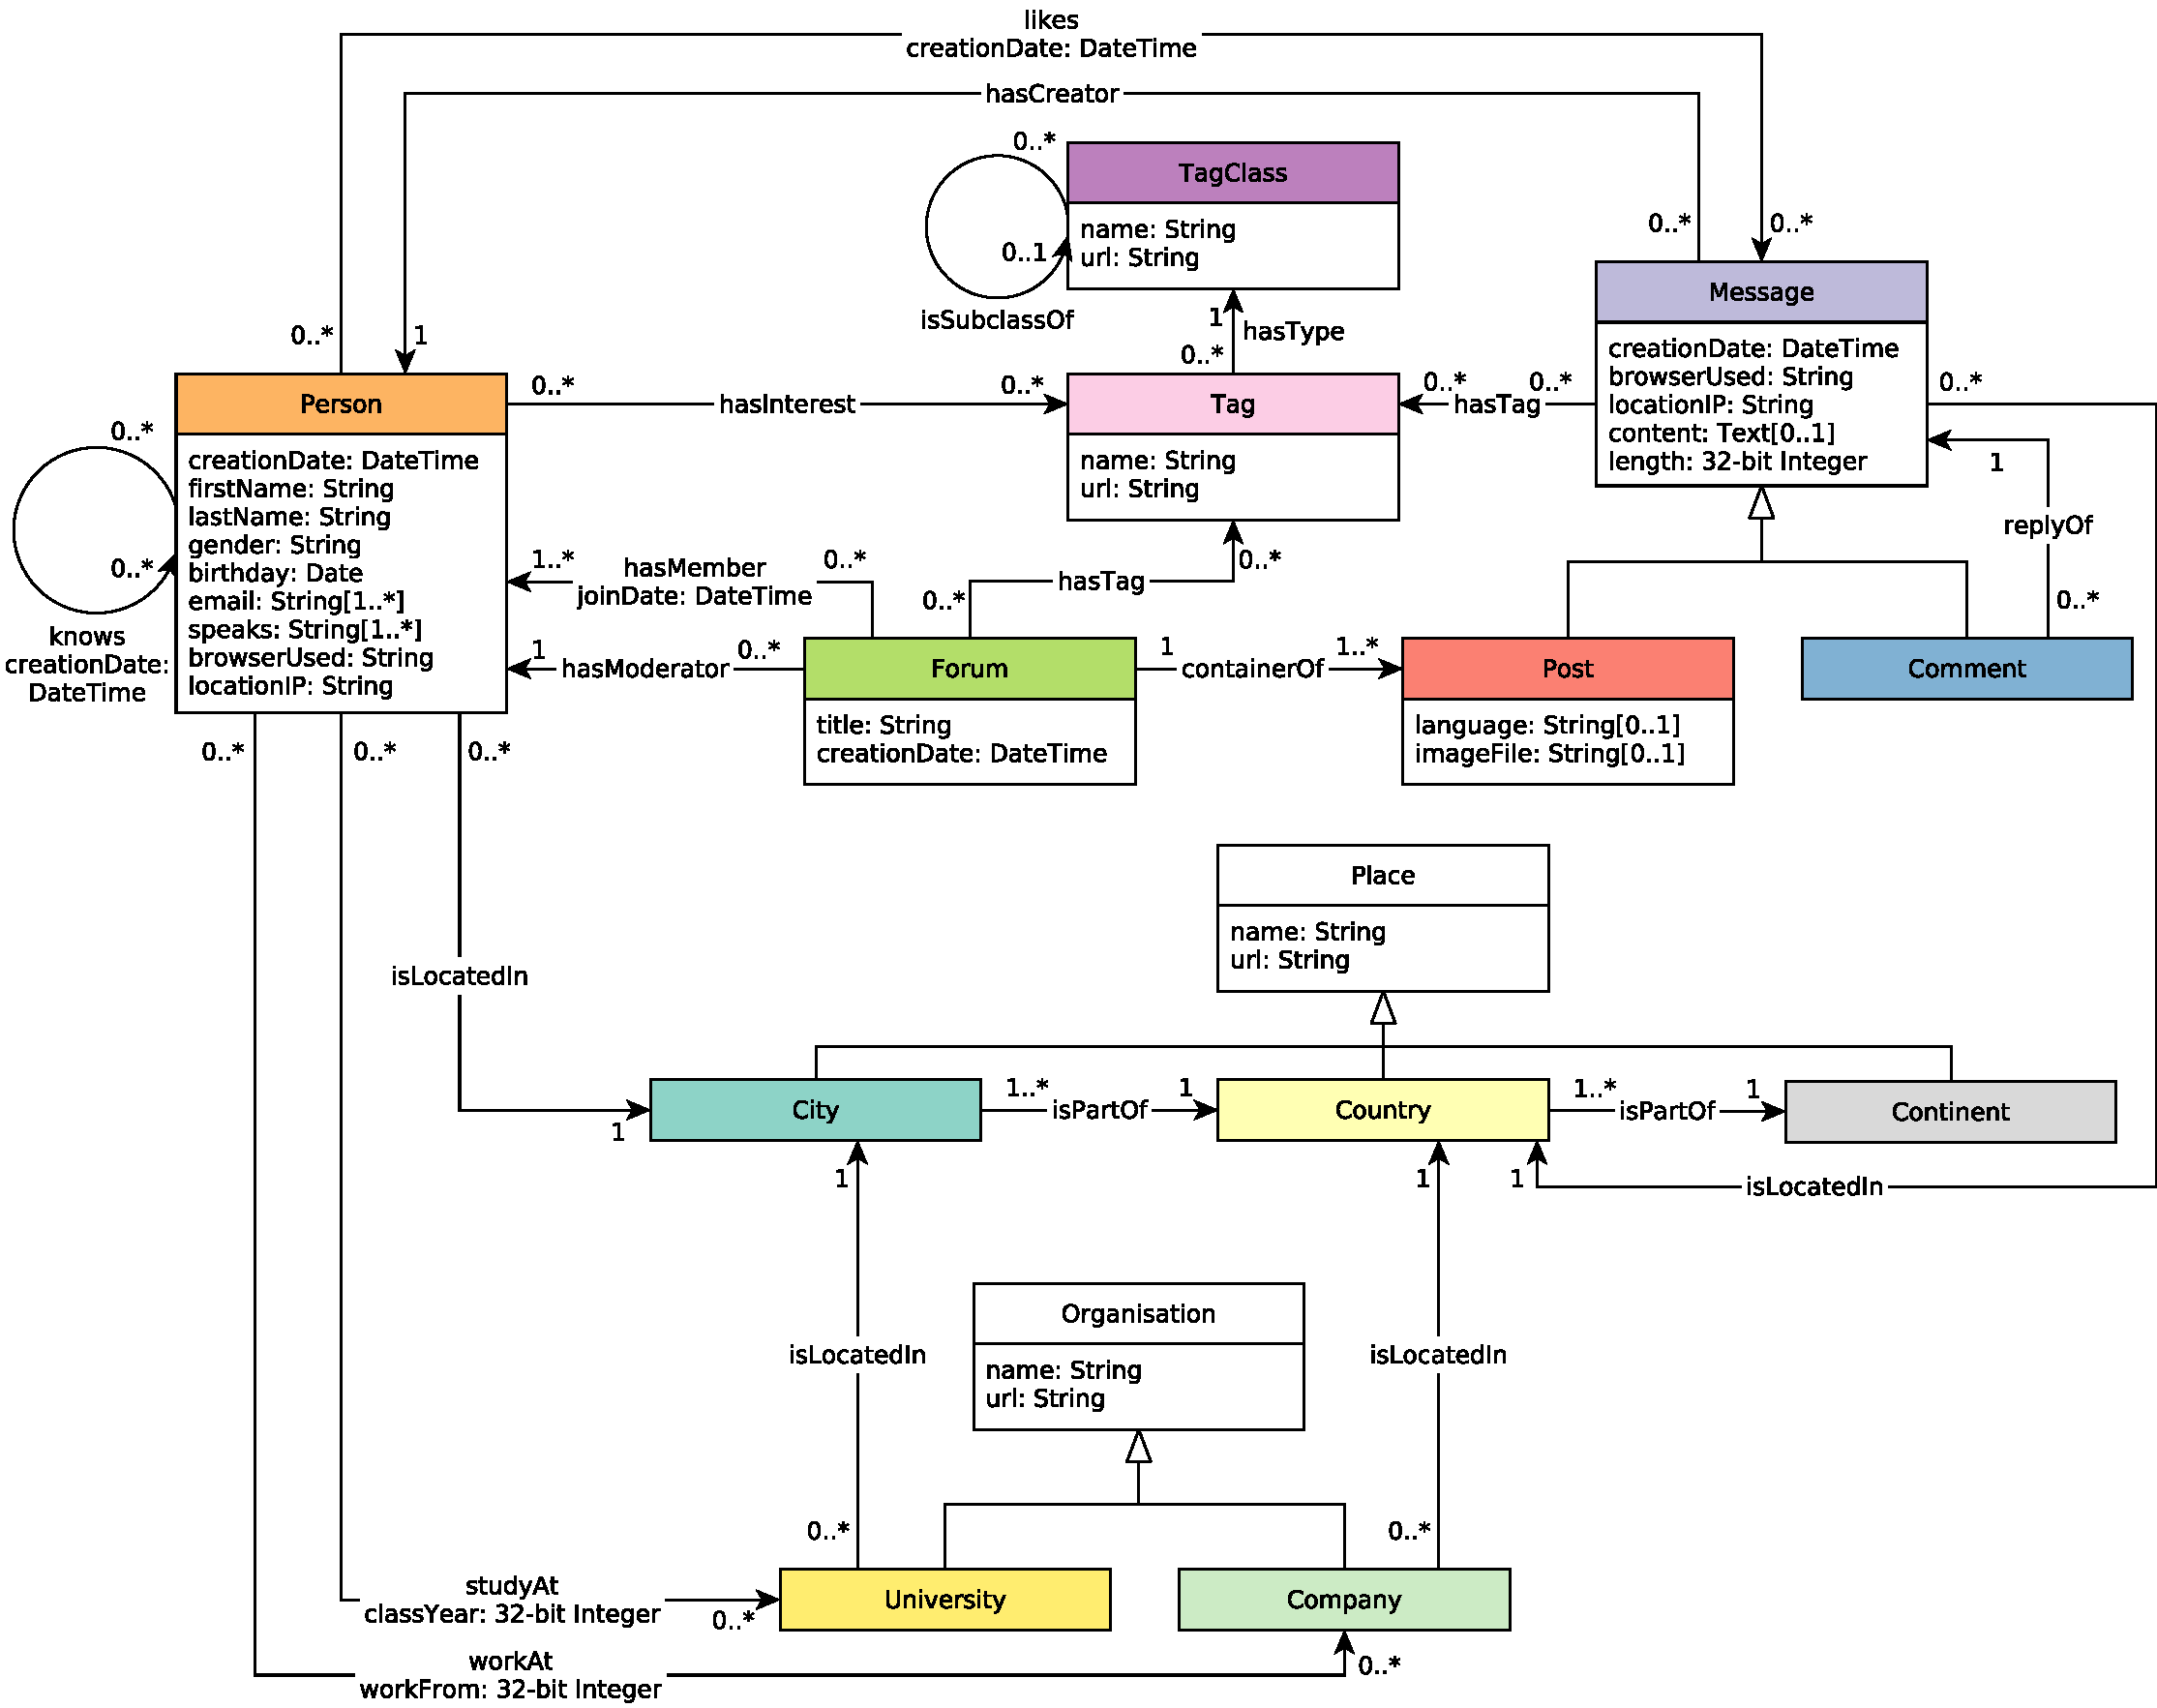
\includegraphics[width=\linewidth]{schema.pdf}
	\caption{Az LDBC Social Network Benchmark gráf sémája}
	\label{fig:dataschema}
\end{figure}

\section{Q1 lekérdezés differenciális adatfolyama}
\label{sec:q1-ddf}

\begin{figure}[h]
	\centering
	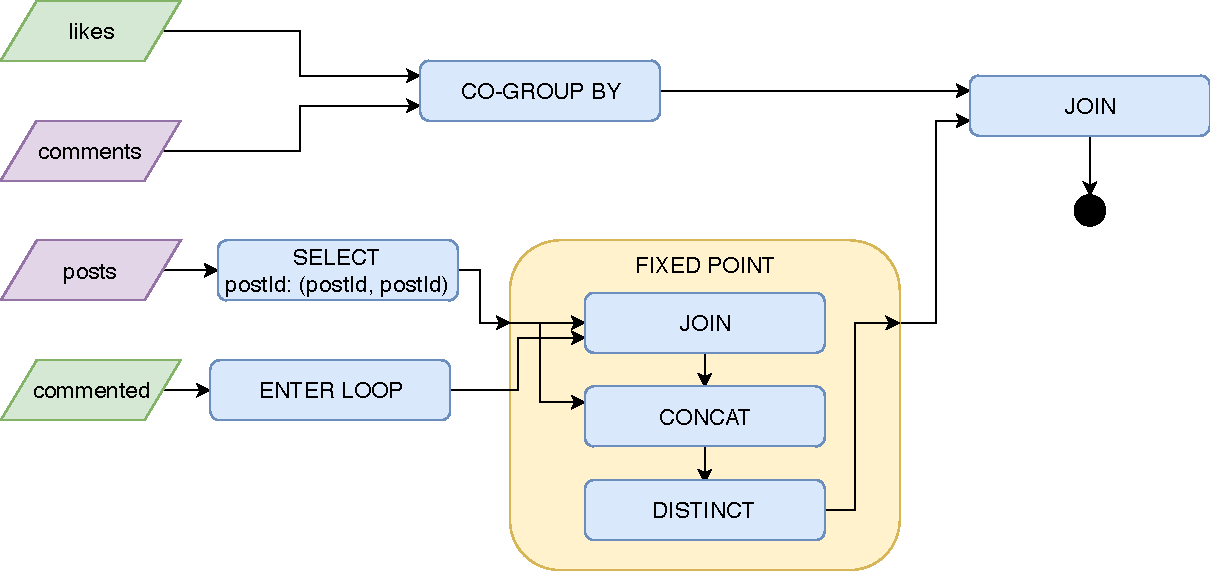
\includegraphics[width=\linewidth]{task1.pdf}
	\caption{A TTC Social Network feladat Q1 lekérdezésének differenciális adatfolyama}
	\label{fig:q1-ddffig}
\end{figure}